% Copyright (c)  2019  FSC.
% Permission is granted to copy, distribute and/or modify this document
% under the terms of the GNU Free Documentation License, Version 1.3
% or any later version published by the Free Software Foundation;
% with no Invariant Sections, no Front-Cover Texts, and no Back-Cover Texts.
% A copy of the license is included in the section entitled "GNU
% Free Documentation License".

\chapter{Web Design}\label{chap:web-design}
In questo capitolo viene illustrata la fase di web design.

Nel dettaglio, vengono mostrati i diagrammi relativi alla mappa del sito, gli 
storyboad delle pagine e i relativi prototipi di navigazione.

\section{Mappa del sito}\label{sec:mappa-sito}
La seguente mappa è la rappresentazione dei percorsi di navigazione del sito in 
un contesto generale.

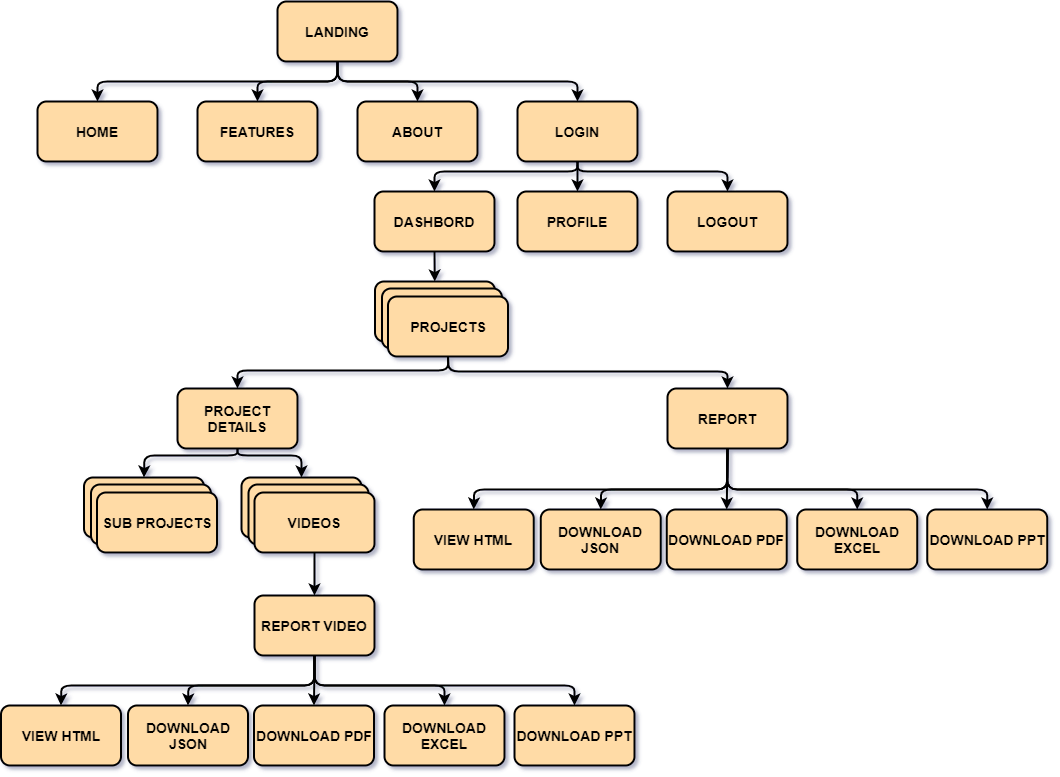
\includegraphics[width=\linewidth]{images/mappa-sito.png}

\section{Storyboard}\label{sec:storyboard}
Gli storyboard sono la rappresentazione di particolari sequenze di navigazione 
del sito, accompagnata da una sintetica descrizione.

% Copyright (c)  2019  FSC.
% Permission is granted to copy, distribute and/or modify this document
% under the terms of the GNU Free Documentation License, Version 1.3
% or any later version published by the Free Software Foundation;
% with no Invariant Sections, no Front-Cover Texts, and no Back-Cover Texts.
% A copy of the license is included in the section entitled "GNU
% Free Documentation License".

\begin{figure}[H]
	\centering
	\caption{Storyboard del login.}
	\label{fig:storyboard:login}
	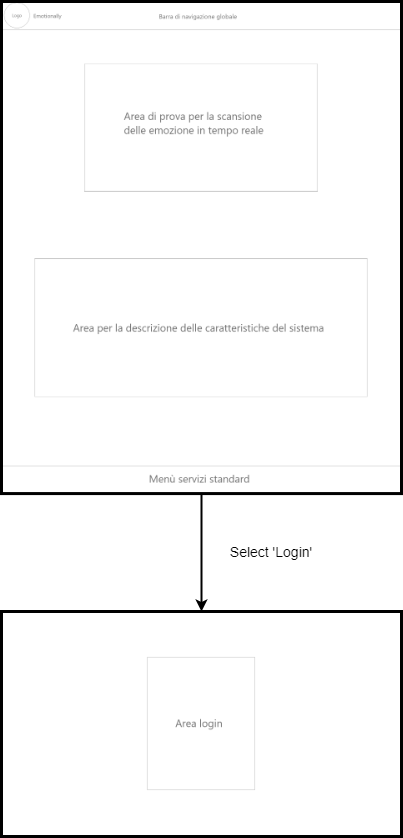
\includegraphics[width=\textwidth]{images/storyboard/login}
\end{figure}

\begin{figure}[H]
	\centering
	\caption{Storyboard della registrazione.}
	\label{fig:storyboard:sign-up}
	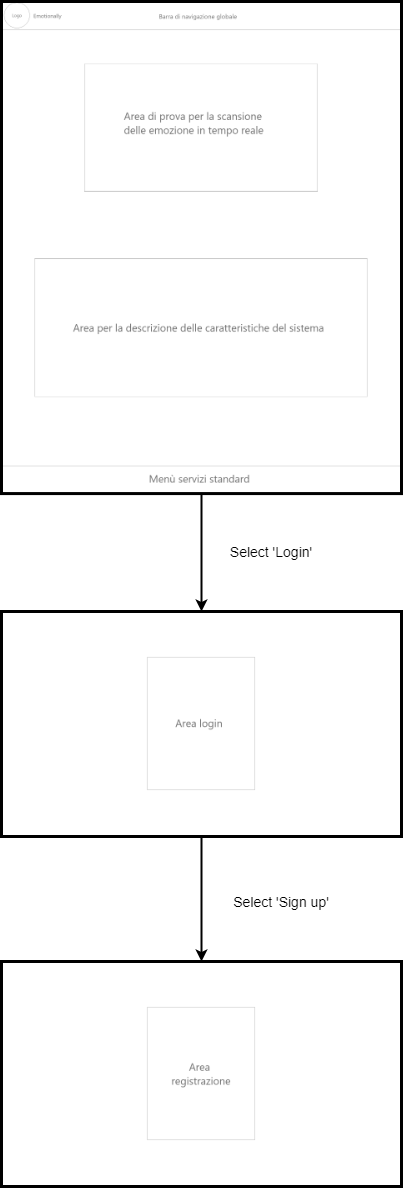
\includegraphics[width=\textwidth]{images/storyboard/sign-up}
\end{figure}
\begin{figure}[H]
	\centering

	\caption{Storyboard della dashboard}
	\label{fig:storyboard:dashboard}
	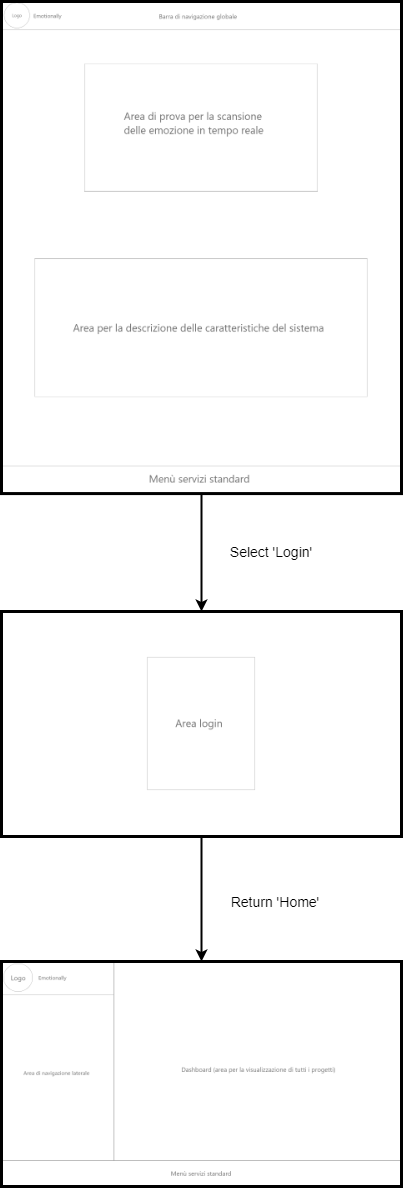
\includegraphics[width=\textwidth]{images/storyboard/dashboard}
\end{figure}

\begin{figure}[H]
	\centering
	\caption{Storyboard della visualizzazione dei dettagli di un progetto.}
	\label{fig:storyboard:project}
	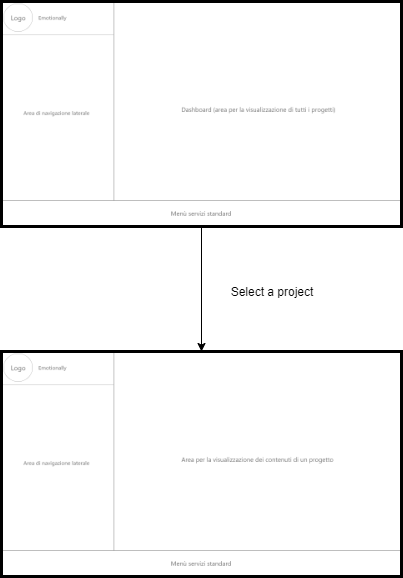
\includegraphics[width=\textwidth]{images/storyboard/project}
\end{figure}

\begin{figure}[H]
	\centering
	\caption{Storyboard della visualizzazione del report di un progetto.}
	\label{fig:storyboard:report-project}
	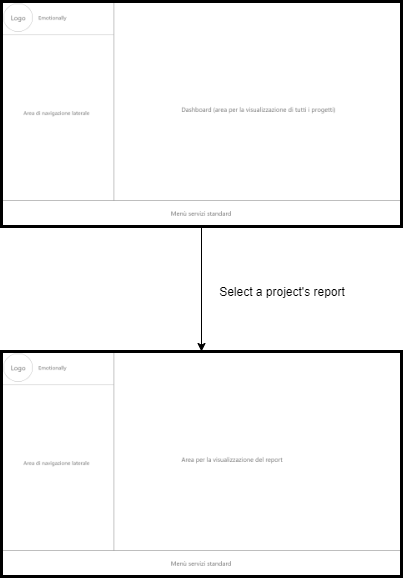
\includegraphics[width=\textwidth]{images/storyboard/report-project}
\end{figure}

\begin{figure}[H]
	\centering
	\caption{Storyboard della visualizzazione del report di un video.}
	\label{fig:storyboard:report-video}
	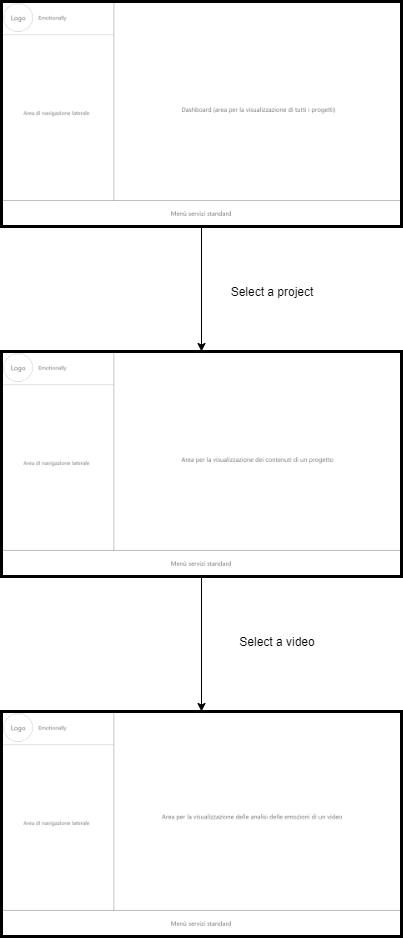
\includegraphics[width=\textwidth]{images/storyboard/report-video}
\end{figure}

\begin{figure}[H]
	\centering
	\caption{Storyboard della visualizzazione del profilo.}
	\label{fig:storyboard:profilo}
	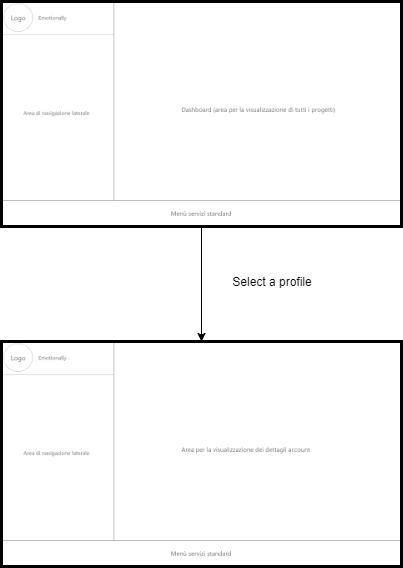
\includegraphics[width=\textwidth]{images/storyboard/profile}
\end{figure}


\section{Prototipo di navigazione}\label{sec:prototipo-navigazione}
È un prototipo piuttosto rudimentale completamente navigabile. Le pagine sono 
costituite dalla sola gabbia logica, in bianco e nero, senza grafica, senza 
contenuti informativi e il <<testo fittizio>> inserito nella gabbia logica.

% Copyright (c)  2019  FSC.
% Permission is granted to copy, distribute and/or modify this document
% under the terms of the GNU Free Documentation License, Version 1.3
% or any later version published by the Free Software Foundation;
% with no Invariant Sections, no Front-Cover Texts, and no Back-Cover Texts.
% A copy of the license is included in the section entitled "GNU
% Free Documentation License".

\begin{figure}[H]
	\centering
	\caption{Gabbia logica della pagina di login.}
	\label{fig:gabbie-logiche:login}
	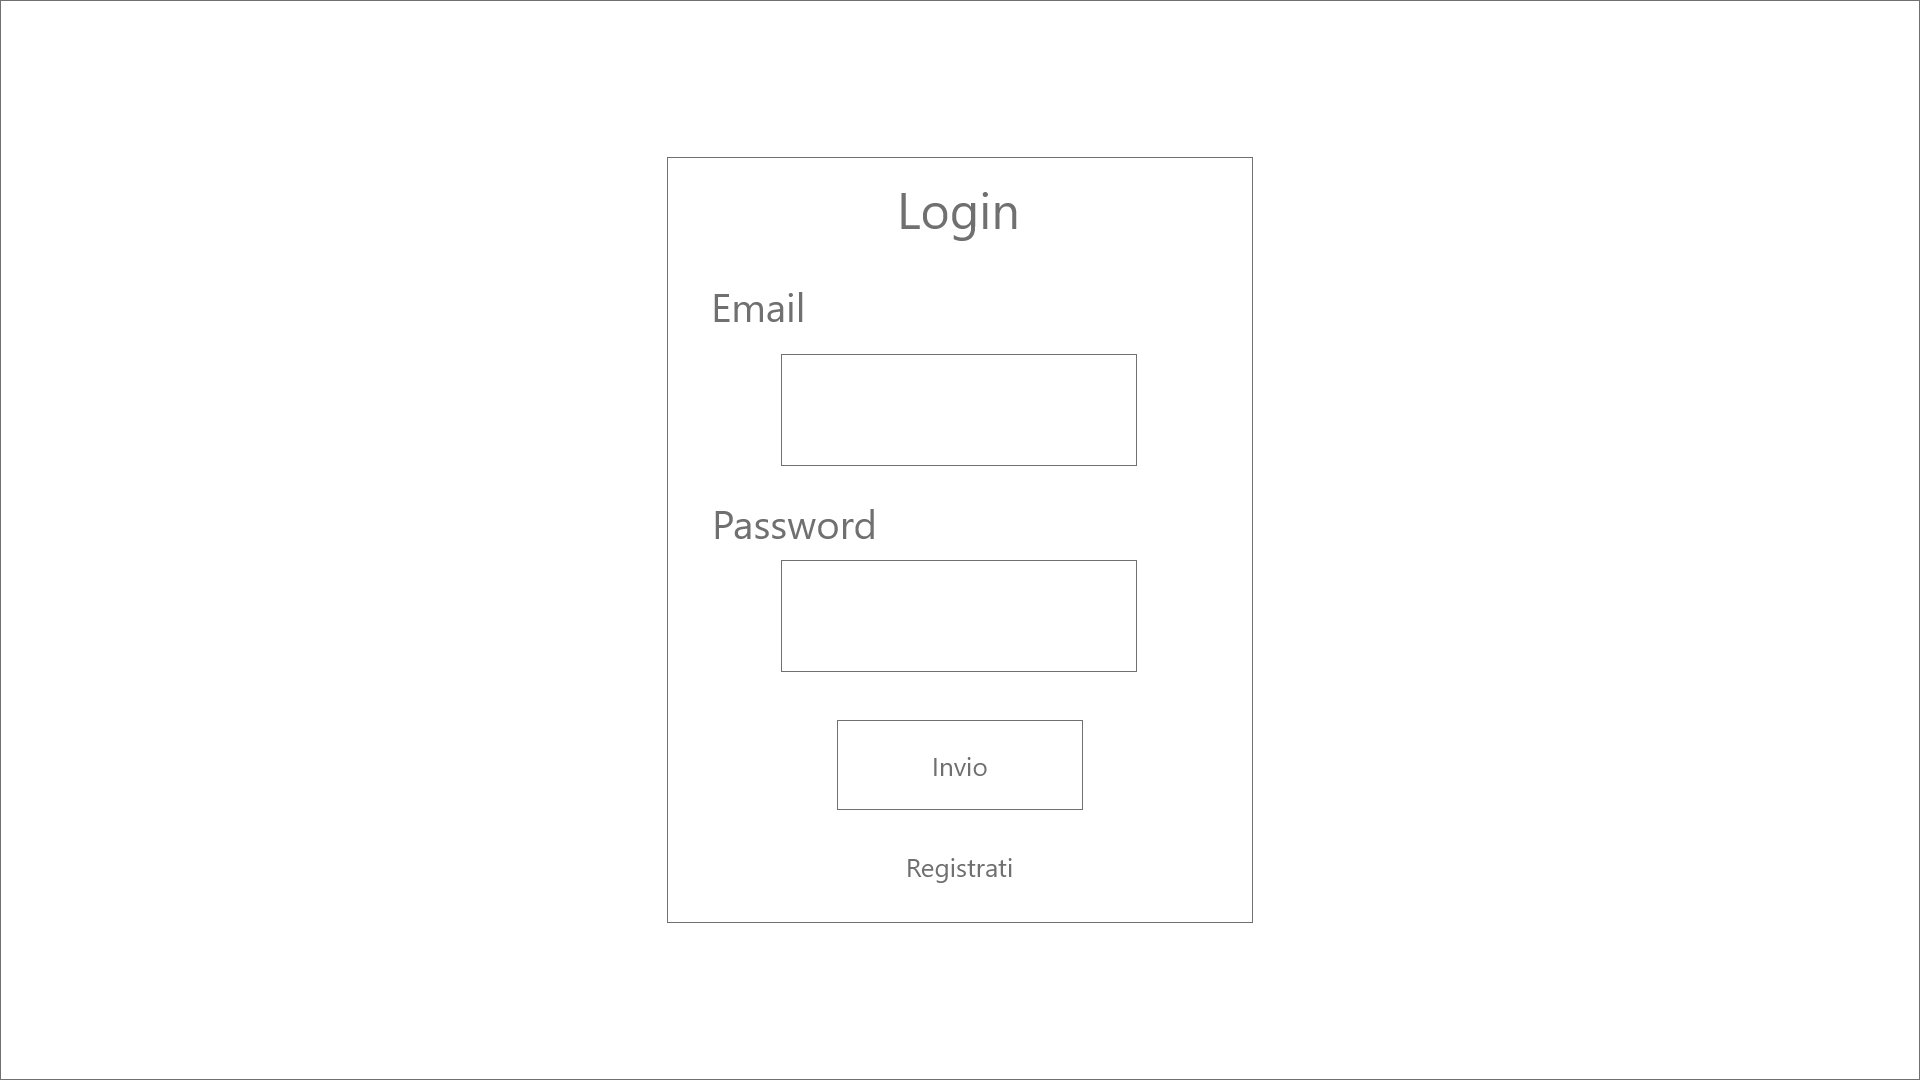
\includegraphics[width=\textwidth]{images/gabbie-logiche/Login}
\end{figure}

\begin{figure}[H]
	\centering
	\caption{Gabbia logica della landing page.}
	\label{fig:gabbie-logiche:landing-page}
	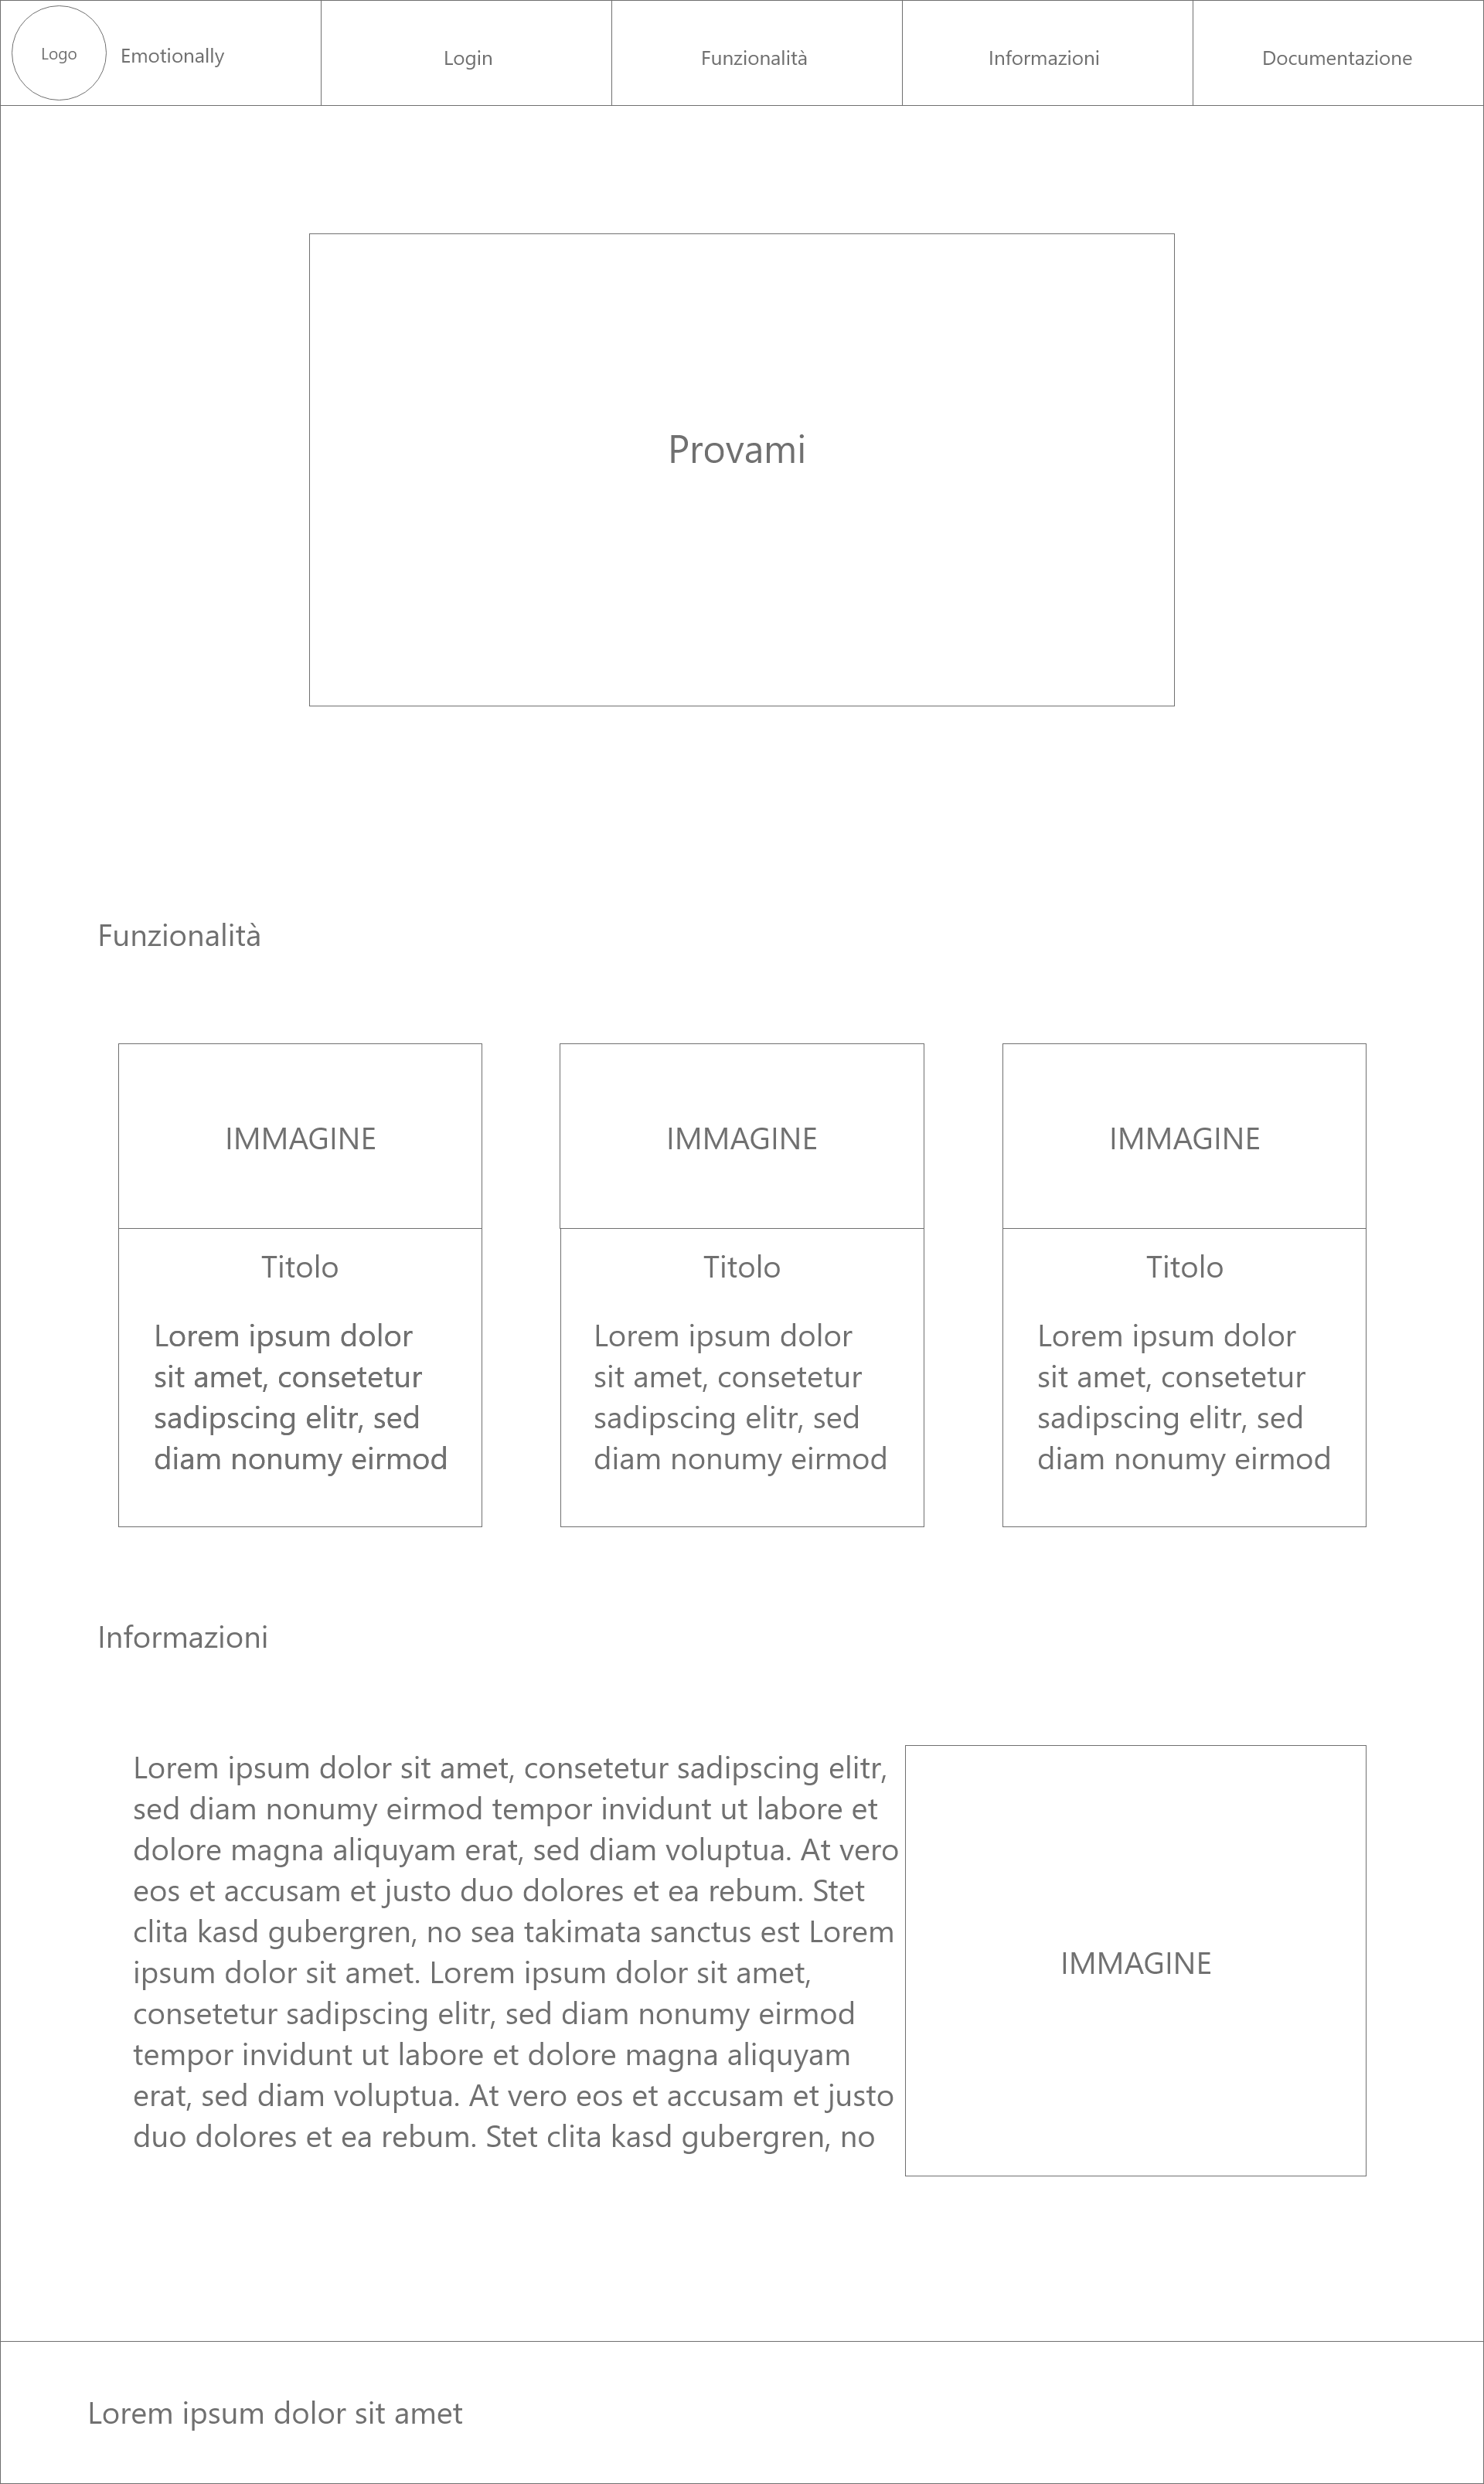
\includegraphics[height=\textheight-3ex]{images/gabbie-logiche/Landing}
\end{figure}

\begin{figure}[H]
	\centering

	\caption{Gabbia logica della pagina di registrazione.}
	\label{fig:gabbie-logiche:registrazione}
	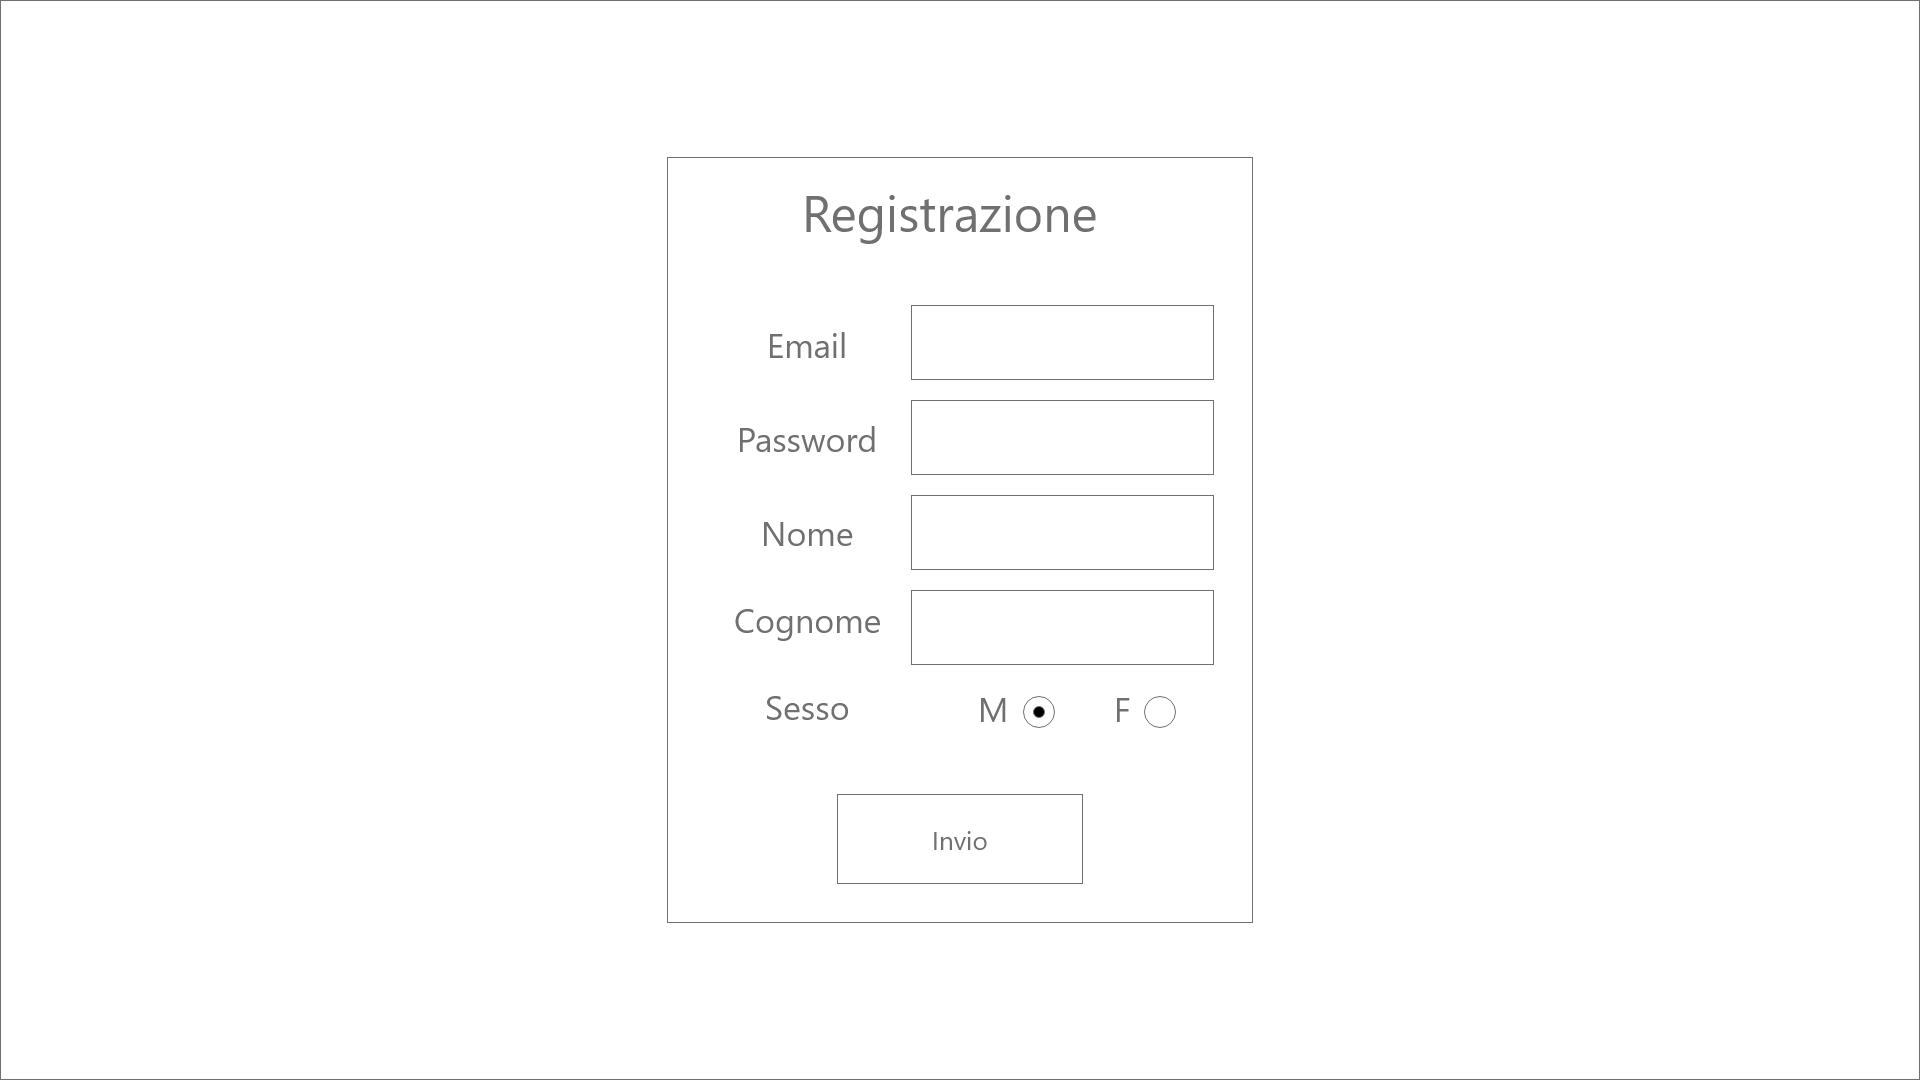
\includegraphics[width=\textwidth]{images/gabbie-logiche/Registrazione}
\end{figure}

\begin{figure}[H]
	\centering
	\caption{Gabbia logica della home page.}
	\label{fig:gabbie-logiche:home-page}
	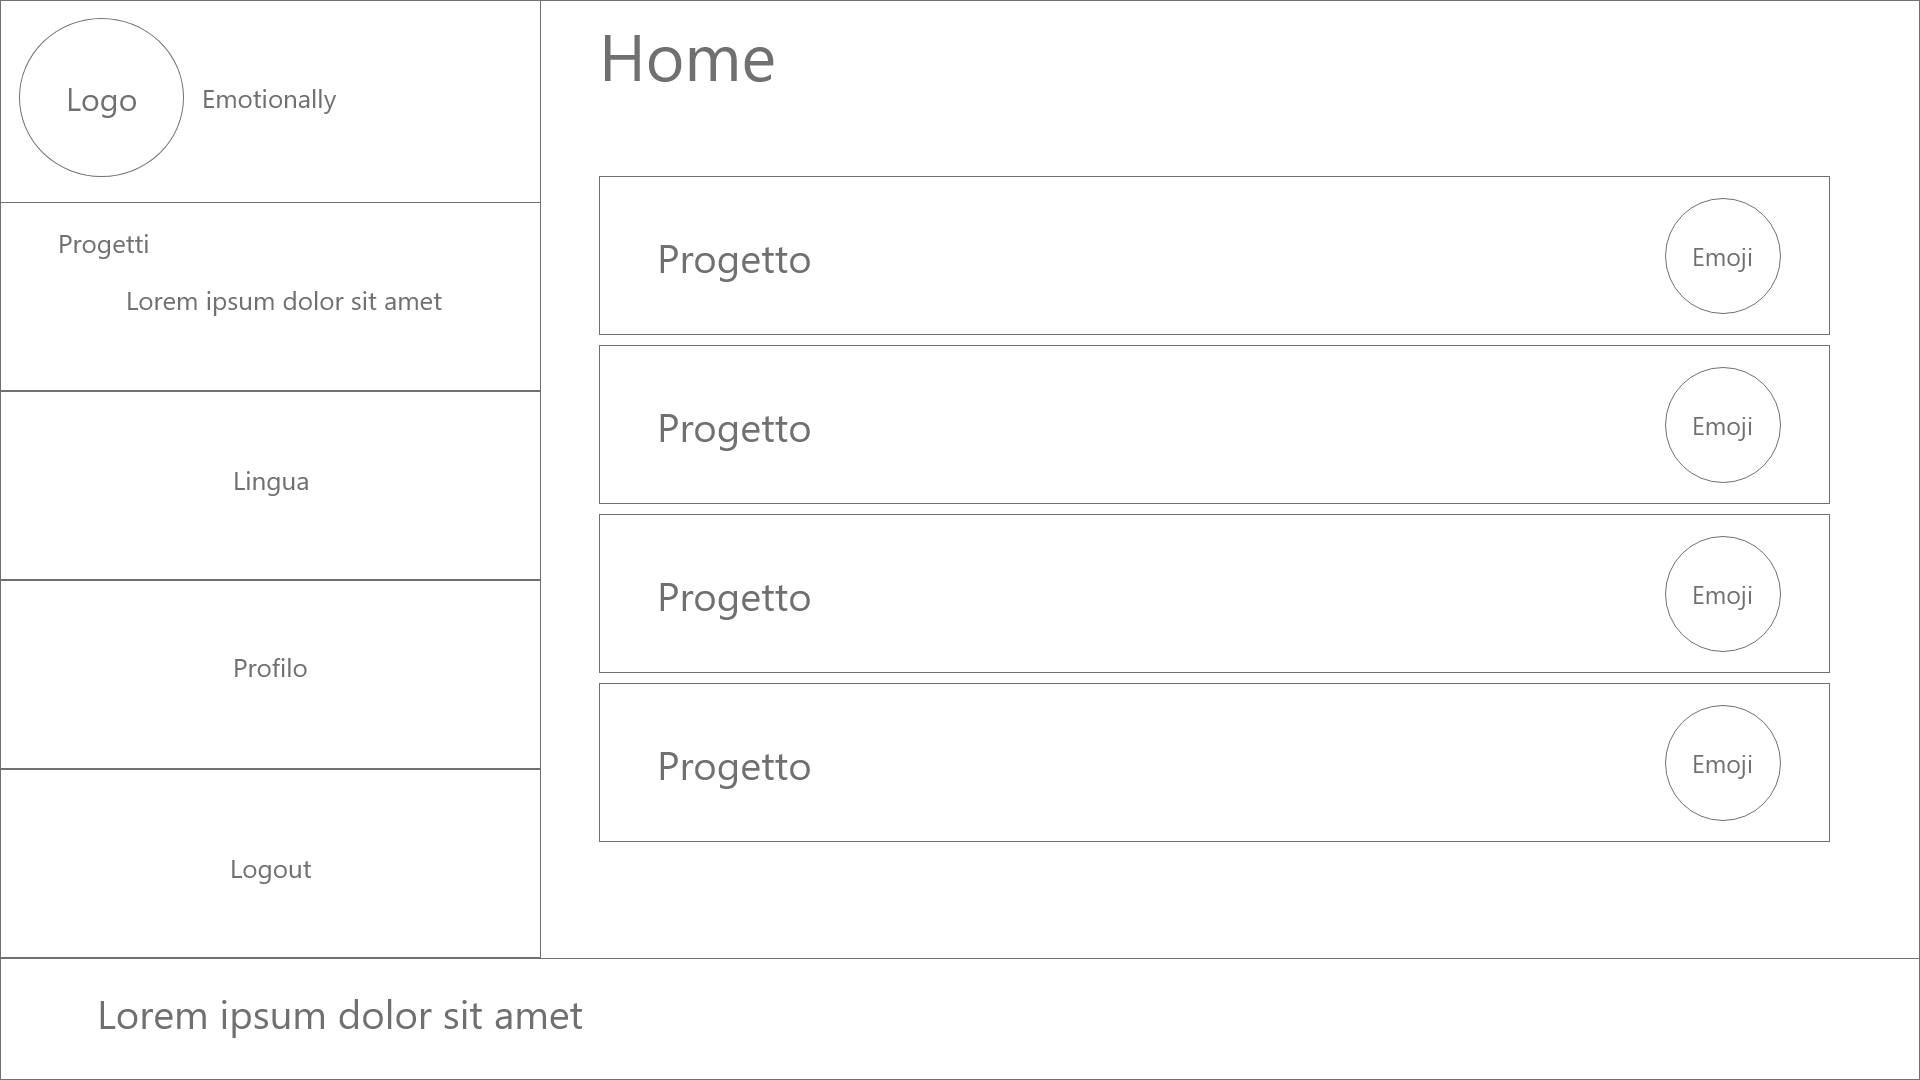
\includegraphics[width=\textwidth]{images/gabbie-logiche/Home}
\end{figure}

\begin{figure}[H]
	\centering
	\caption{Gabbia logica della pagina di un progetto.}
	\label{fig:gabbie-logiche:project}
	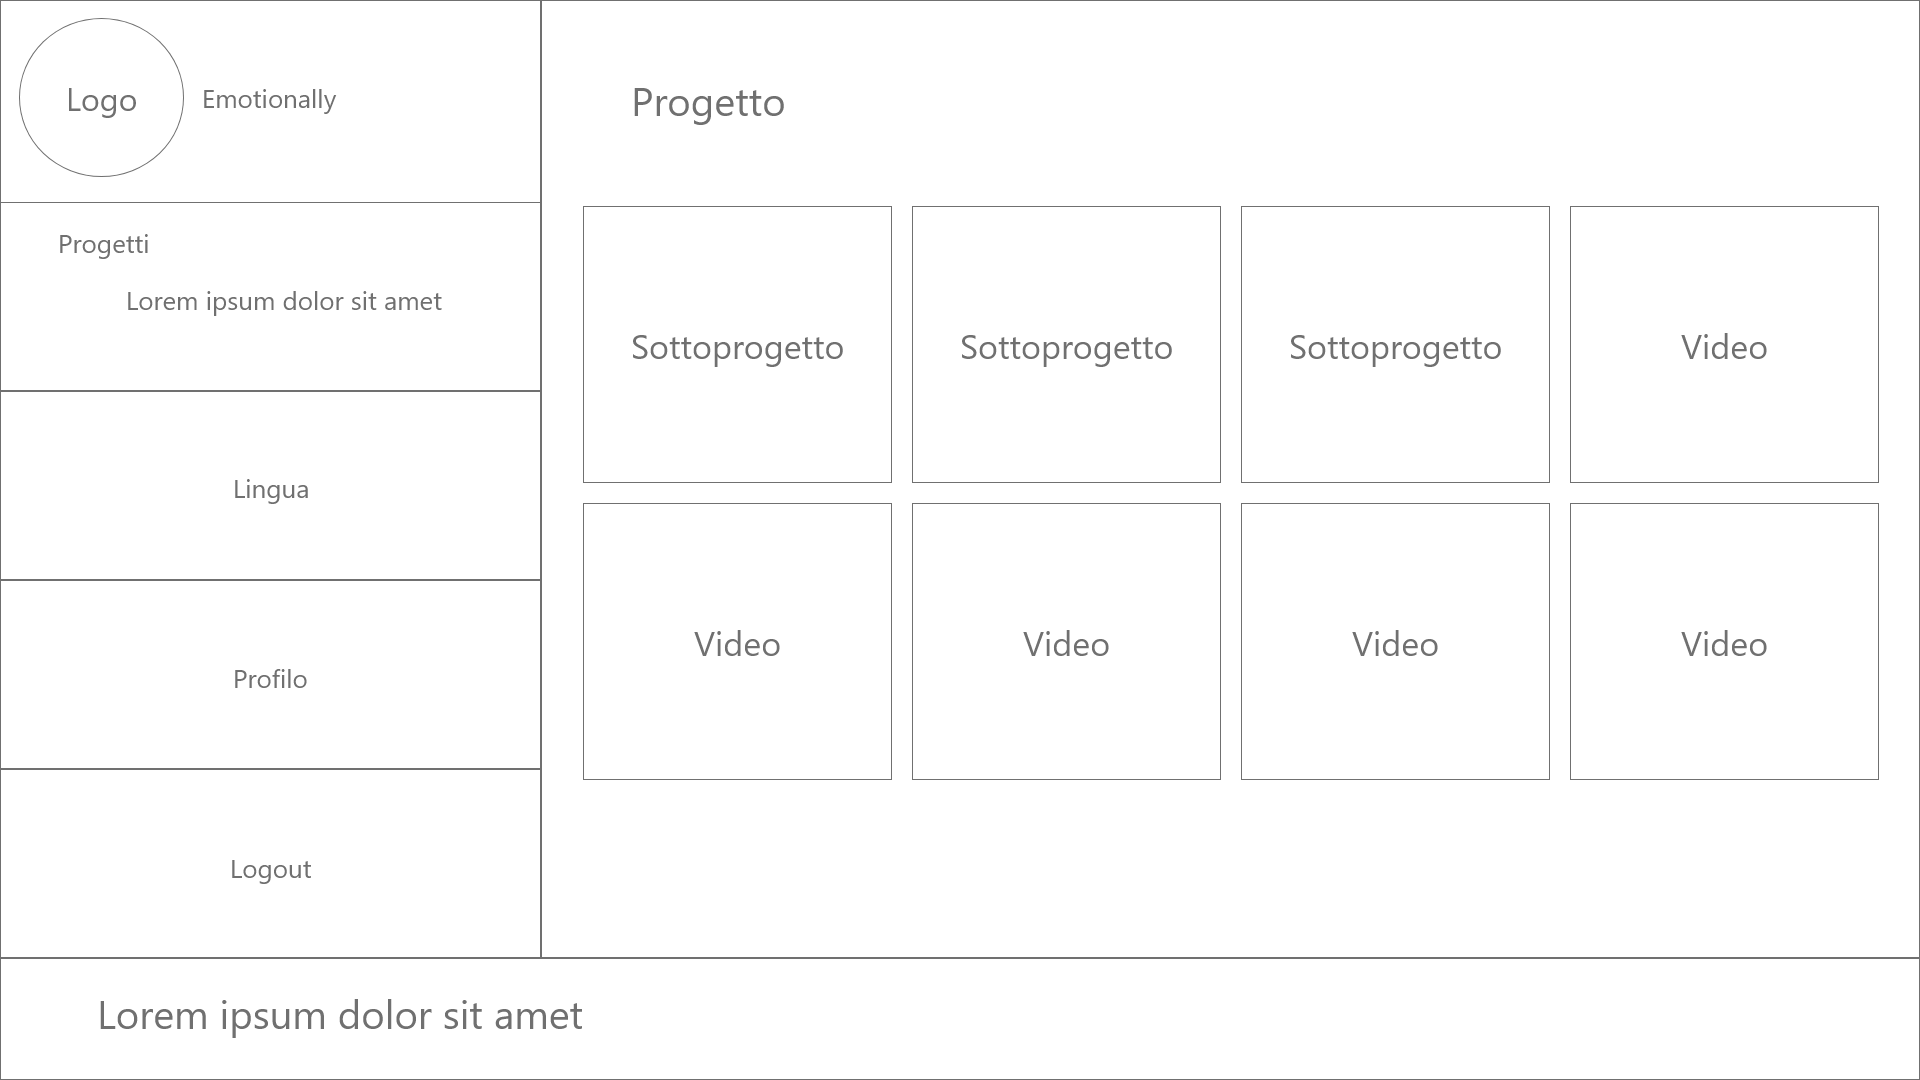
\includegraphics[width=\textwidth]{images/gabbie-logiche/Progetto}
\end{figure}

\begin{figure}[H]
	\centering
	\caption{Gabbia logica della pagina di un video.}
	\label{fig:gabbie-logiche:video}
	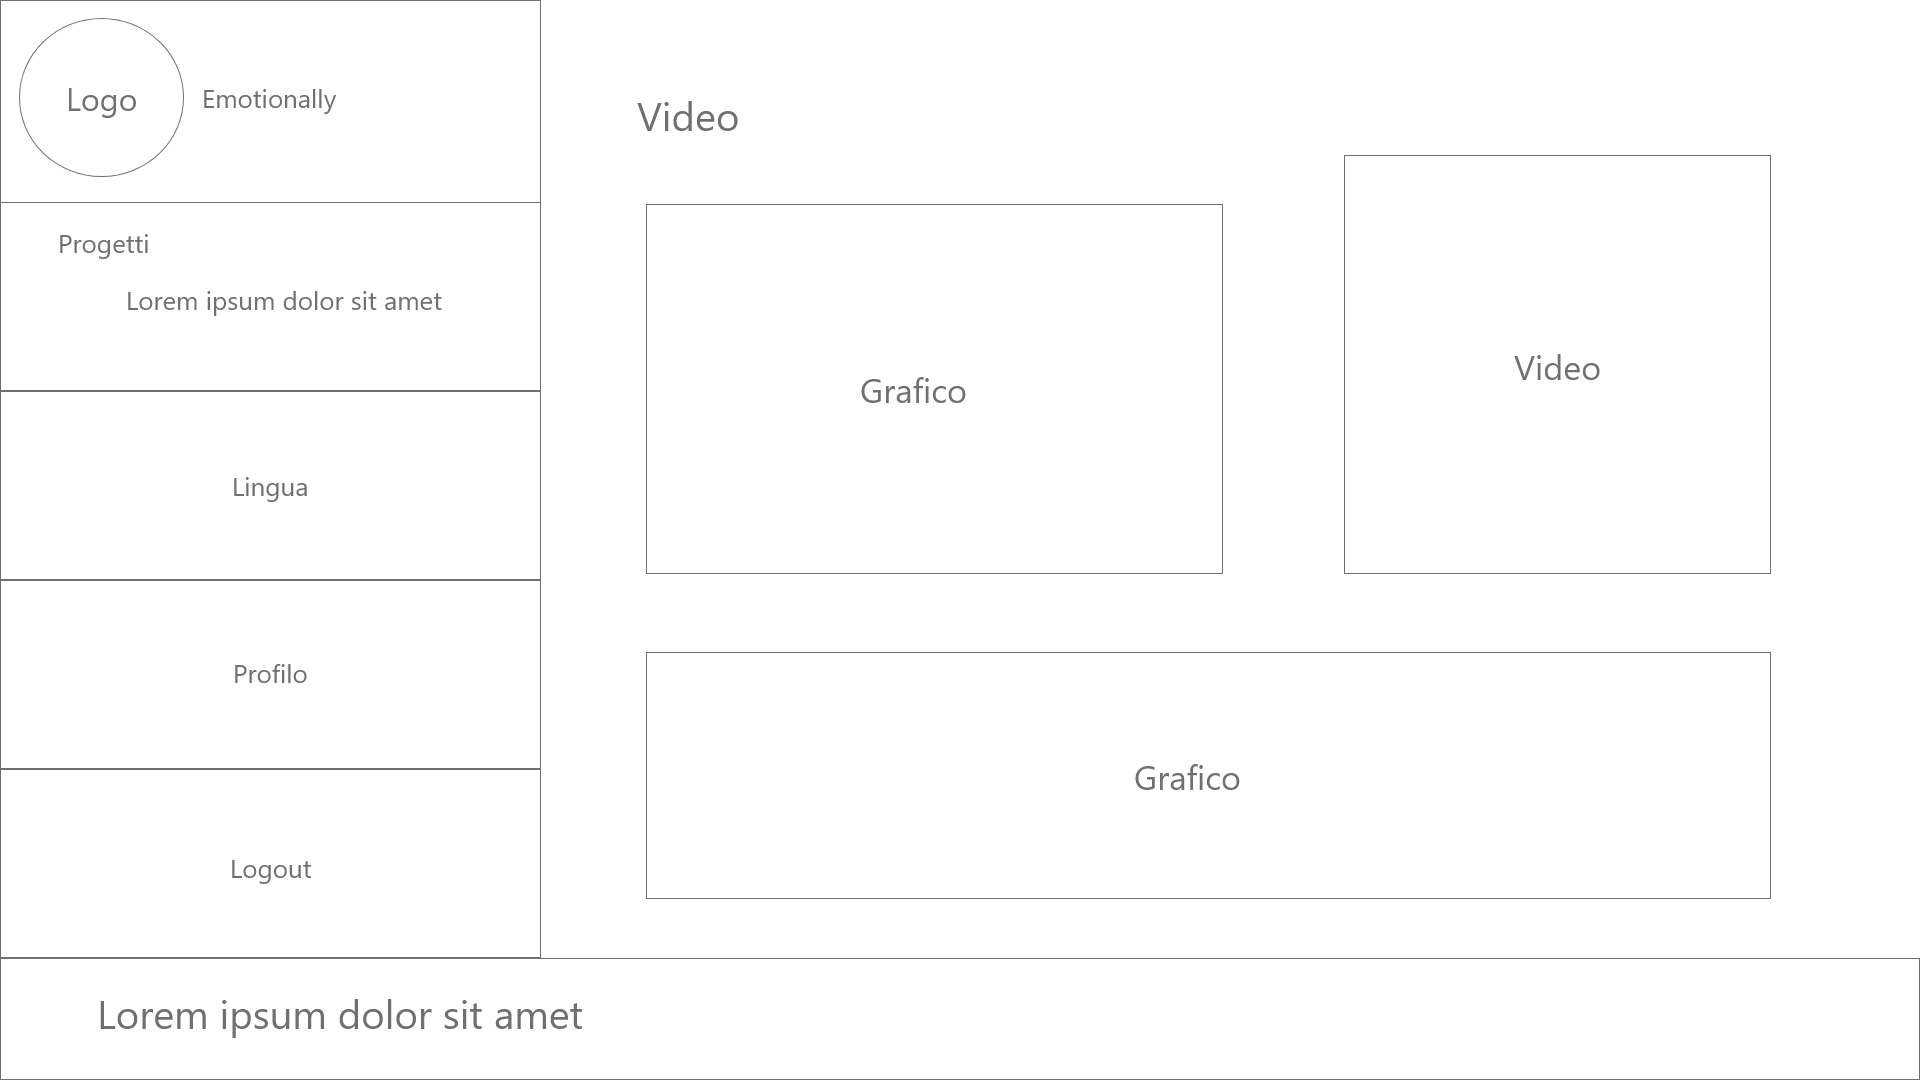
\includegraphics[width=\textwidth]{images/gabbie-logiche/Video}
\end{figure}

\begin{figure}[H]
	\centering
	\caption{Gabbia logica della pagina di profilo.}
	\label{fig:gabbie-logiche:profilo}
	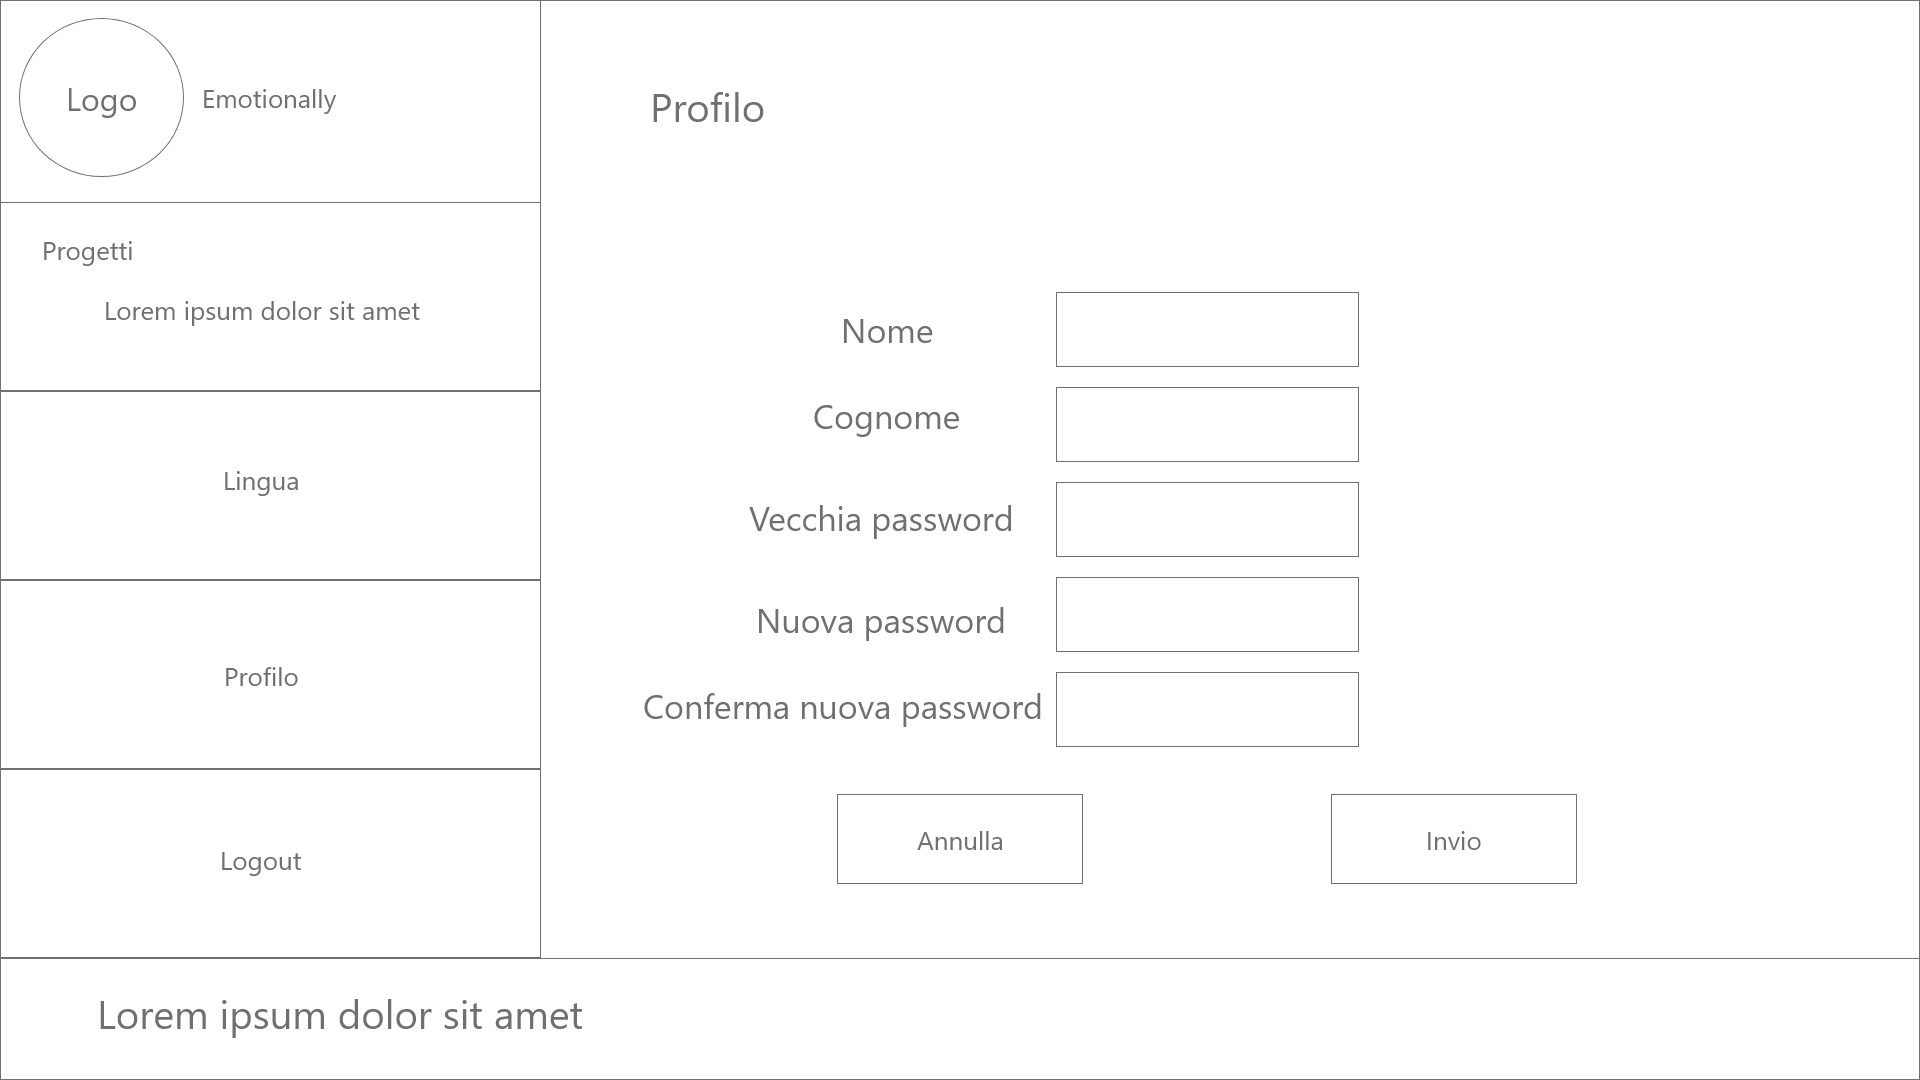
\includegraphics[width=\textwidth]{images/gabbie-logiche/Profilo}
\end{figure}

\begin{figure}[H]
	\centering
	\caption{Gabbia logica della pagina del sottoprogetto.}
	\label{fig:gabbie-logiche:sottoprogetto}
	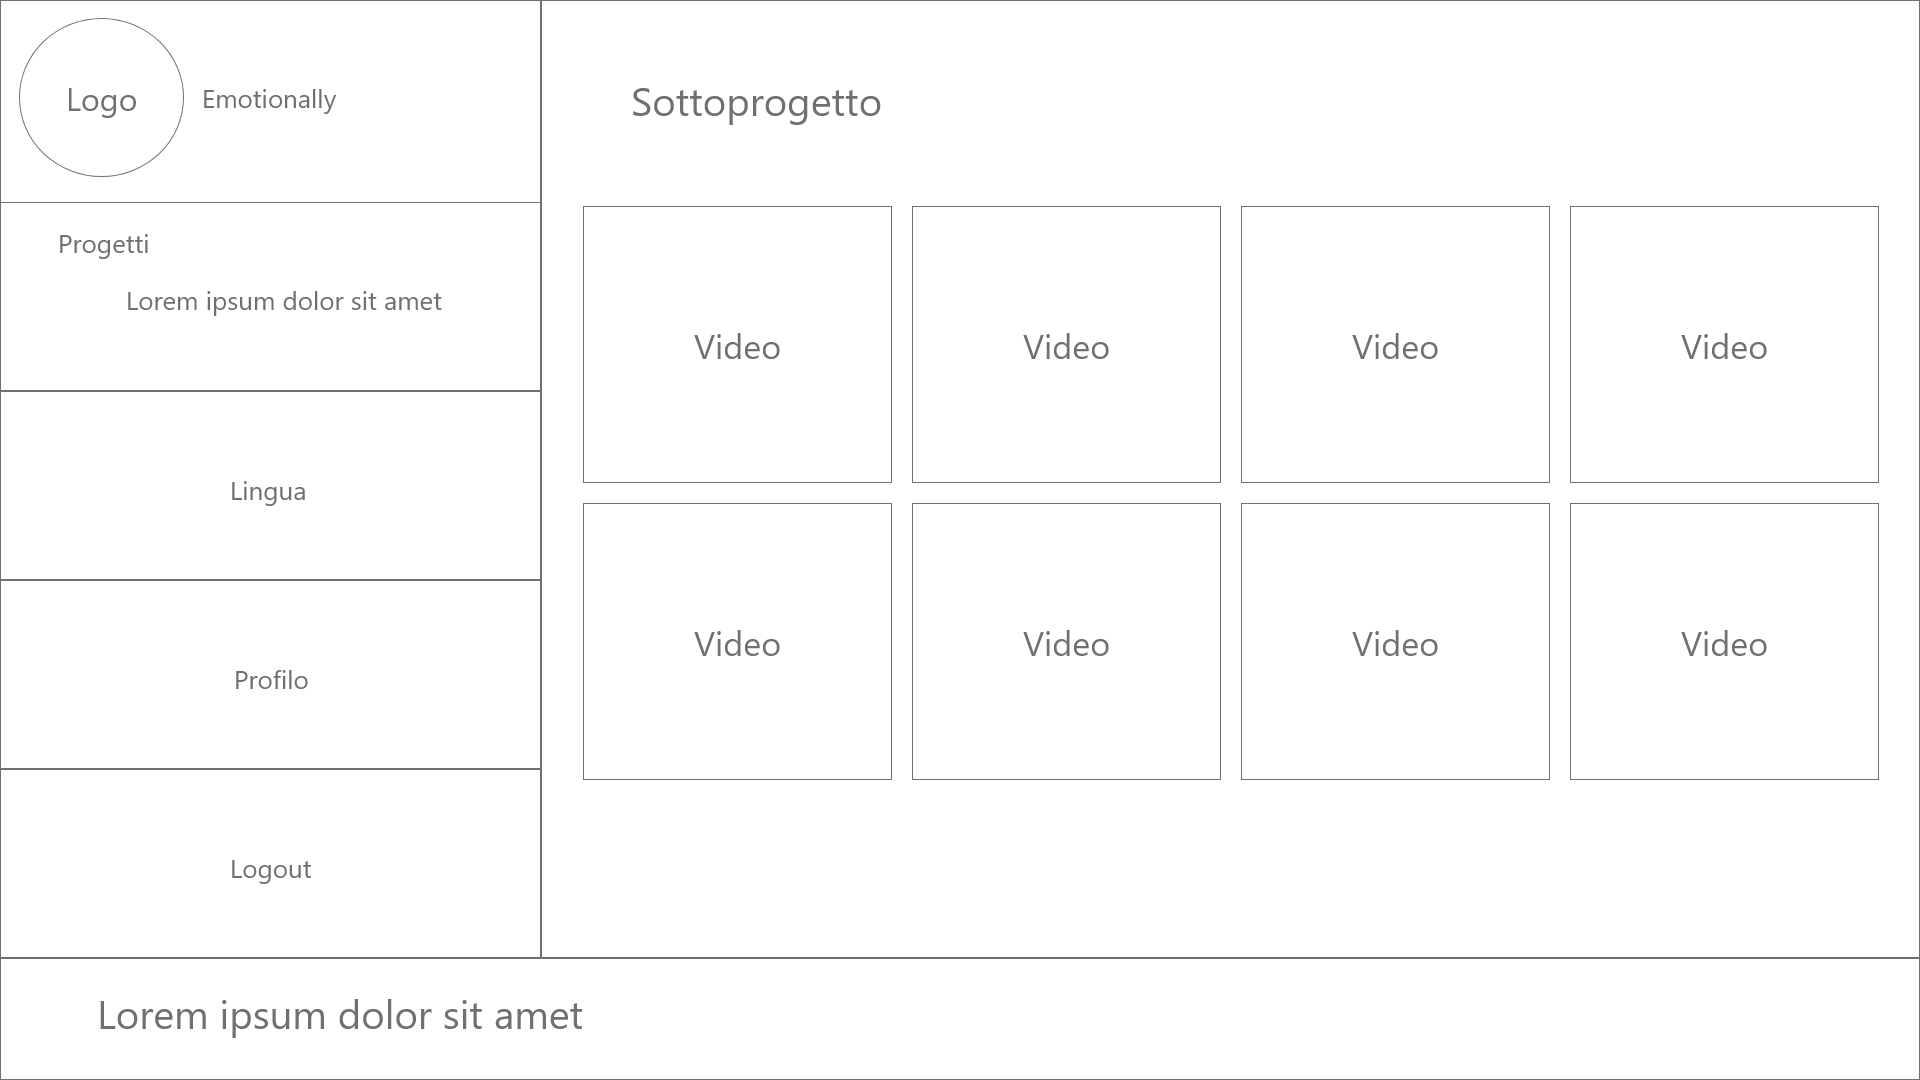
\includegraphics[width=\textwidth]{images/gabbie-logiche/Sottoprogetto}
\end{figure}

